
%(BEGIN_QUESTION)
% Copyright 2007, Tony R. Kuphaldt, released under the Creative Commons Attribution License (v 1.0)
% This means you may do almost anything with this work of mine, so long as you give me proper credit

EIA/TIA-485 networks require {\it biasing resistors} to provide a definite ``idle'' (mark) state when the drivers are all in high-impedance mode.  Otherwise, the lines would be left to float, and the logic state would be indeterminate.

Show how two resistors are connected to the A and B lines inside each EIA/TIA-485 device to provide a definite idle state.  Note that these resistors are usually internal to the device, and do not have to be externally added:

$$\includegraphics[width=15.5cm]{i02195x01.eps}$$

\vskip 20pt \vbox{\hrule \hbox{\strut \vrule{} {\bf Suggestions for Socratic discussion} \vrule} \hrule}

\begin{itemize}
\item{} How would the presence of {\it termination} resistors affect this biasing?
\end{itemize}


\underbar{file i02195}
%(END_QUESTION)





%(BEGIN_ANSWER)

Pulling B high and A low places an otherwise floating differential line into the idle (1, off, or mark) state.

$$\includegraphics[width=15.5cm]{i02195x02.eps}$$

%(END_ANSWER)





%(BEGIN_NOTES)

With a (low-valued) termination resistor at either (or both) end of the cable, the bias resistor network would be greatly affected!  Here is a comparative circuit to illustrate:

$$\includegraphics[width=15.5cm]{i02195x03.eps}$$

The impact is especially pronounced because $R_{term} << R_{bias}$.

\vskip 10pt

On an entirely different note, the location of the shield ground is entirely arbitrary: I could have just as well placed it on the left-hand shield terminal.  So long as I terminate only one end of the cable's shield, it will work properly.

%INDEX% Networking, bias resistors: EIA/TIA-485
%INDEX% Networking, signal voltages: EIA/TIA-485

%(END_NOTES)


